\section{Q-Learning}

Q-learning\cite{watkins1992q} is a a model-free reinforcement learning algorithm which estimate a value for each (state, action) pair
and with these estimated values compute a policy that can maximize the expected discounted reward.

Given S a set of states of the environments, A a set of agents's possible actions,
$\pi$ : SxAxS $\rightarrow$ [0, 1] a function which gives the probability of reaching state s' while agent is in the state s and perform the action a,
r : SxAxS $\rightarrow$ $\mathbb{R}$ a function which gives the amount of reward the agent will receive when perform the action a while in state s and move to state s',
the cumulative discounted reward can be defined as $R_t = \sum_{i=0}^{\infty} \gamma^i r_{t+k+1}$
where $\gamma$ $\in$ [0, 1] is the discount factor which makes futures rewards less valuable than the current ones.

The algorithm, therefore, has a function that calculates the quality of a pair (state, action): $Q:S\times A\to {\mathbb  {R}}.$
update formula: $Q(s_t, a_t) \leftarrow Q(s_t, a_t) + \alpha [r_{t+1} + \gamma \max_a Q(s_{t+1}, a) - Q(s_t, a_t)]$ where alpha is the learning rate.

``an agent tries an action at a particular state, and evaluates its consequences in terms of the immediate reward or penalty
it receives and its estimate of the value of the state to which it is taken''\cite{watkins1992q}.
``By trying all actions in all states repeatedly, it learns which are best overall, judged by long-term discounted reward''\cite{watkins1992q}.

Given a finite Markov Decision Process, infinite exploration time and a partly-random policy
the Q-learning algorithm is able to learn an optimal action-selection policy.

A problem of this method is the limitation of the state-action space required, that can be partially solved with an approximation function.
instead of storing each Q-values a mapping function could be learned to map a state-action pair to their respective Q-value.

\subsection{SARSA}

SARSA algorithm\cite{qiang2011reinforcement} is a variation of the Q-learning algorithm. Its name come from $(s, a, r, s', a')$, that are $(state, action, reward, state', action')$, and they are used to compute the update.

An algorithm has an "Off-Policy" technique if it learns the value function according to the action derived from another policy. On the other hand, it called "On-Policy" if it learns the value function according to the current action derived from the current policy.
Q-learning has an Off-Policy technique while SARSA has an On-Policy one.

The update formula of SARSA is similar to the one used by the Q-learning: $Q(s_t, a_t) \leftarrow Q(s_t, a_t) + \alpha [r_{t+1} + \gamma Q(s_{t+1}, a) - Q(s_t, a_t)]$.

This means that SARSA updates the state based on the action taken, while Q-learning updates following the optimal policy.
Suppose to be in a "cliff world", where the agent has to walk from the starting cell to the goal cell along the edge of a cliff without falling off. Q-learning, following the optimal policy, would tend to be close to the edge of the cliff while SARSA would prefer a "safer" path.

\begin{figure}[ht]
    \centering
    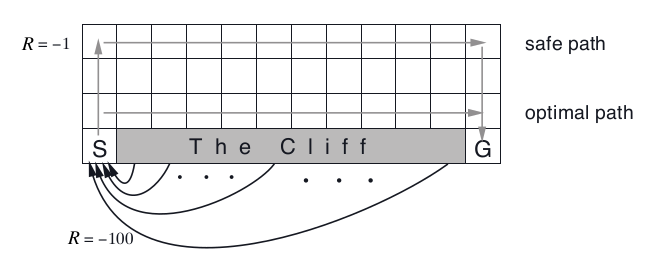
\includegraphics[scale=0.4]{images/cliff_word.png}
    \caption{Image to show the difference between SARSA and Q-learning in a "cliff word".}
    \label{fig:cliff_word}
\end{figure}
